\documentclass[tikz,border=1.35mm]{standalone}

\definecolor{fvmadaptedge}{HTML}{8A7E7E}
\usetikzlibrary{arrows.meta}

\definecolor{externalface}{HTML}{8FB9E8}

% Octahedron / square-bipyramid diamond cell. This six-vertex,
% eight-triangular-face cell appears when pyramid-like pieces meet at a
% quadrilateral midsection.
\begin{document}
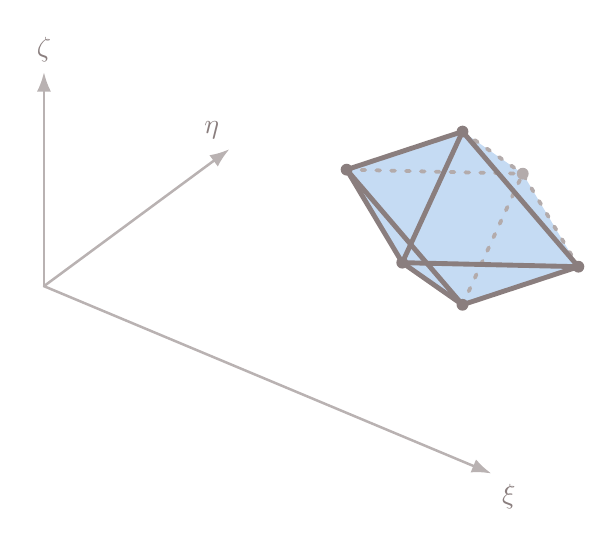
\begin{tikzpicture}[
  x={(20.3mm,-8.5mm)},
  y={(15.3mm,11.3mm)},
  z={(0mm,20mm)},
  line join=round,
  line cap=round,
  outer/.style={draw=fvmadaptedge,line width=0.62mm},
  hidden/.style={draw=fvmadaptedge!65,line width=0.48mm,loosely dotted},
  face/.style={fill=externalface,fill opacity=0.30,draw=none},
  axis/.style={draw=fvmadaptedge!60,line width=0.32mm,-{Latex[length=2.5mm,width=1.8mm]}}
]
  % Equator vertices lie in the middle zeta plane; T and S are the upper and
  % lower apices of the octahedron.
  \coordinate (L) at (0,0.5,0.55);
  \coordinate (F) at (0.725,0,0.55);
  \coordinate (R) at (1.45,0.5,0.55);
  \coordinate (B) at (0.725,1,0.55);
  \coordinate (T) at (0.725,0.5,1.10);
  \coordinate (S) at (0.725,0.5,0);

  % Offset computational-coordinate axes.
  \coordinate (Oaxis) at (-1.20,-0.42,-0.18);
  \draw[axis] (Oaxis) -- (1.60,-0.42,-0.18) node[below right,font=\normalsize,text=fvmadaptedge] {$\xi$};
  \draw[axis] (Oaxis) -- (-1.20,1.12,-0.18) node[above left,font=\normalsize,text=fvmadaptedge] {$\eta$};
  \draw[axis] (Oaxis) -- (-1.20,-0.42,1.18) node[above,font=\normalsize,text=fvmadaptedge] {$\zeta$};

  % Exterior triangular faces. Draw the far faces first, then nearer faces.
  \path[face] (T) -- (B) -- (L) -- cycle;
  \path[face] (S) -- (B) -- (L) -- cycle;
  \path[face] (T) -- (R) -- (B) -- cycle;
  \path[face] (S) -- (R) -- (B) -- cycle;
  \path[face] (T) -- (L) -- (F) -- cycle;
  \path[face] (S) -- (L) -- (F) -- cycle;
  \path[face] (T) -- (F) -- (R) -- cycle;
  \path[face] (S) -- (F) -- (R) -- cycle;

  % Hidden far-side edges.
  \draw[hidden] (L) -- (B) -- (R);
  \draw[hidden] (T) -- (B);
  \draw[hidden] (S) -- (B);

  % Visible exterior wireframe.
  \draw[outer] (L) -- (F) -- (R);
  \draw[outer] (T) -- (L);
  \draw[outer] (T) -- (F);
  \draw[outer] (T) -- (R);
  \draw[outer] (S) -- (L);
  \draw[outer] (S) -- (F);
  \draw[outer] (S) -- (R);

  % Original vertices are #8a7e7e, with the back equator vertex softened.
  \foreach \p in {L,F,R,T,S} {
    \fill[fvmadaptedge] (\p) circle[radius=0.75mm];
  }
  \fill[fvmadaptedge!65] (B) circle[radius=0.75mm];
\end{tikzpicture}
\end{document}
